
% parts of the intro...
\textcolor{red}{change to focus on tree diseases}
Since humans society diverted away from a hunter-gather lifestyle and transitioned to agricultural-based communities (the neolithic revolution), wide-spread epidemics have been an ever-present threat. Population mixing, high-density communities and the raising of livestock upset natural equilibrium states between host and pathogen. The neolithic revolution lead to densely packed areas in close proximity to other species brought and disease could travel rapidly through communities due to high densities and were more prevalent due to the accumulation of human and livestock waste.

Epidemiology has a rich history routed in both superstition and religiosity. The first objective theory of disease came from the Greek physician Hippocrates (460\---370 BC) \citep{garrison1922introduction}. Over the ages, models and understanding of communicable disease have been refined and various theory's put forward pioneers.

Modernity has witnessed not only epidemics within human populations but also within plant species. \textcolor{red}{Talk and link above paragraph to trees}. 
The first equation based mathematical model of disease, the $SIR$ model, was developed by \cite{kermack-model}, canonically named the `Kermack-Mckendrick model'. As we shall see $SIR$-type models are still used extensively in the $21^{st}$ century and will form an underlying component of the models developed in this thesis. As such, a brief description of the equations and results of the Kermack-Mckendrick model will be given in \ref{sec:sir-kmc}.

% talk about computational models
\section{Computational Implementation}

Computationally modelling a physical process first began during World War 2, scientists modelled nuclear detonation in a large scale collaboration. Since then, the advent of ever increasing computational power has lead to vast amounts of research and scientific understanding. In recent epidemiological research, epidemiologists have taken advantage of modern computer power to simulate disease progression in order to study both applied and theoretical problems. This project will focus on using cellular automata as the main class of computational model. Cellular automata were first developed to model John von Neumann's idea of self-replicating machines\---a Von Neumann universal constructor \cite{NEUMANN_MACHINE}. Von Neumann's idea was to design a machine which both replicated itself and could simulate a Turing machine, after proving mathematically this was possible he subsequently realised the practical challenge of building such a machine. Following suggestions from Stanislaw Ulam, Von Neumann resolved to simulate this machine on a discrete system giving rise to the Von Neumann cellular automata. The Von Neumann cellular automata is complicated and will not be discussed in detail. A Von Neumann automata can be loosely defined as a spatial pattern on a lattice obeying simple interaction rules which can both self-replicate and simulate any computational algorithm. The basic idea was to first define a lattice on computer memory where each lattice site contains just one state out of a set of possible states, the different states give rise to a pattern when viewed over a larger scale. The lattice sites then interact via simple local rules. Importantly, the interaction rules between sites give rise to a self-replicating pattern. Furthermore, the pattern is capable of simulating the logic of any computer algorithm (or turning machine), such a system of computation is called 'turning complete'.

Developing upon Von Neumann's work lead to various interesting Turing complete models such as Conway's game of life which happen to be much simpler than Von Neumann's cellular automata. Conway's game of life is the archetypical cellular automata model and can be defined using two types of states, alive or dead, existing on a square lattice. Interestingly the time evolution of cellular automata models only depend upon the initial conditions. The interaction rules between nearest neighbours are as follows: 1) A live cell dies if less than two nearest neighbours are alive i.e. underpopulated 2) A live cell dies if more than three nearest neighbours are alive i.e. overpopulation 3) A live cell survives into the next generation if two or three nearest neighbours are alive 4) A dead cell is resurrected if exactly three nearest neighbours are alive i.e. reproduction

\begin{figure}
    \centering
    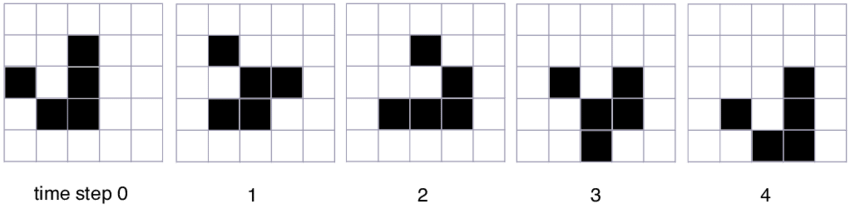
\includegraphics[scale=0.50]{chapter2/figures/game_of_life1.png}
    \caption{A pattern emerges in the game of life cellular automata model, dark and white cells are alive and dead respectively. The pattern seems to mutate whilst propagating from right to left, such patterns are denoted as 'gliders'. Gliders move across the lattice and can be used to transmit information between groups of objects, they can also combine to form more complex objects. This glider demonstrates the emergent property of complex behaviour arising from simple cellular interactions.}
    \label{fig:my_label}
\end{figure}

\begin{figure}
    \centering
    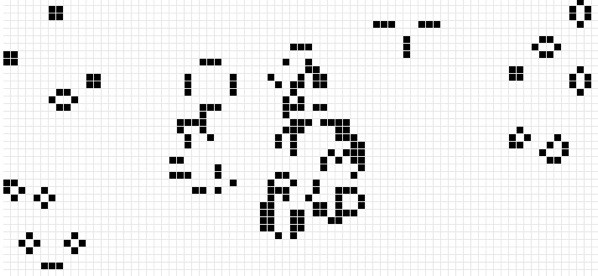
\includegraphics[scale=0.50]{chapter2/figures/game_of_life2.jpg}
    \caption{The game of life in progress. Various patterns and interactions can be seen over the lattice.}
    \label{fig:my_label}
\end{figure}

\begin{figure}
    \centering
    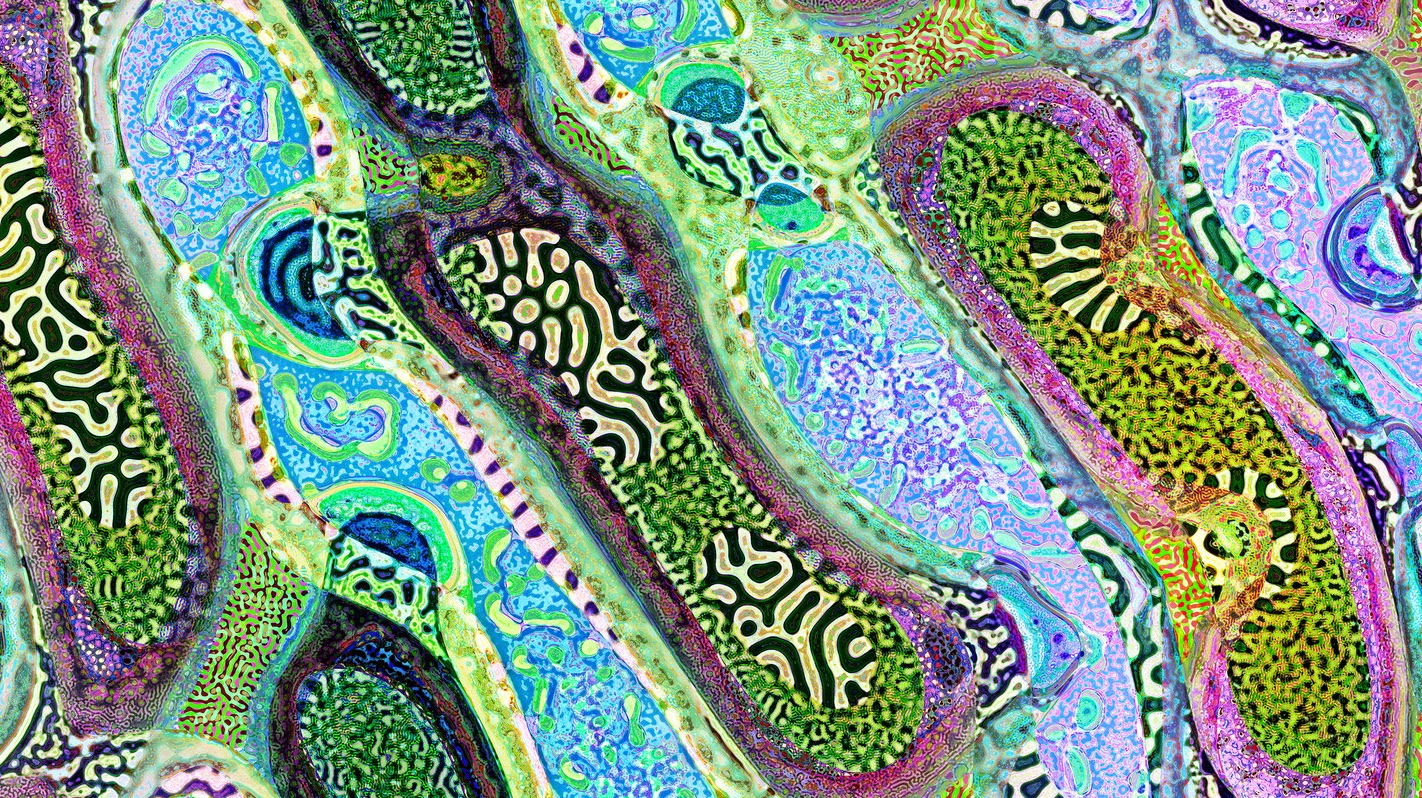
\includegraphics[scale=0.25]{chapter2/figures/cellular_automata.jpg}
    \caption{A cellular automata model given by generative artist Jonathan McCabe. Cellular automata models can give rise to artistic patterns and display a host of complex features such as self organisation and symmetry. }
    \label{fig:my_label}
\end{figure}

Unlike mathematical models such as SIR, modern computational models using cellular automata capture the spatial patterns of disease propagation. In particular, the cellular automata model developed in this project constitute a spatio-temporal lattice model. When viewed through the lens of a stochastic lattice model, the problem of infectious disease can be described by a mean field theory as in statistical mechanics. In recent literature, a mean field theory was derived from a spatio-temporal lattice model of dengue fever \cite{SOUZA_09,SOUZA_13}. From the mean field theory SIR type equations can be derived. It is interesting to note that the corresponding threshold behaviour of $R_0$ corresponds to a phase transition when modelled using a spatio-temporal lattice model.


% talk anout the SIR model...
\section{SIR model\textemdash a primer on compartmentalisation}
\label{sec:sir-kmc}

A model of infectious disease should capture the main processes and behaviour which govern the temporal evolution of an outbreak within a population. The model first developed for mobile human populations \citep{kermack-model} used a coupled set of ODE's to describe the states of susceptible hosts $S$, infected hosts $I$ and removed (or recovered) hosts $R$. These fields obey the following equations:

\begin{align}
\label{eq:sir1}
\frac{dS}{dt}&=  -\beta S I \\
\frac{dI}{dt} &=  \beta S I - \alpha I \\
\frac{dR}{dt} &= \alpha I 
\label{eq:sir3}
\end{align}

One can identify the process $S\rightarrow I \rightarrow R$ governed by the constants $\beta$ and $\alpha$ representing transition rates into the $I$ and $R$ compartments respectively. Initial conditions within the model are set are: $S=N_0$, $I=1$, and $R=0$ where $N_0$ denotes the initial population size. These equations assume each infected individual sufficiently mixes with enough others in the population to seed $\beta N$ new infections per time step\footnote{Later in chapter \textcolor{red}{We will see how this is not satisfied with a localised model of tree disease and how growth rates found in $SIR$ models cannot be fitted.}}, where $N$ is the total population size (mass action incidence). Furthermore, the average removal of infected individuals is given by $\alpha I$ where $\alpha$ is the removal constant. The population size remains constant with respect to births and deaths, fixed as $N=N_0$ and the timescale for epidemic is taken to be faster than the rate of births and deaths in the human host population. 

\begin{figure}
    \centering
    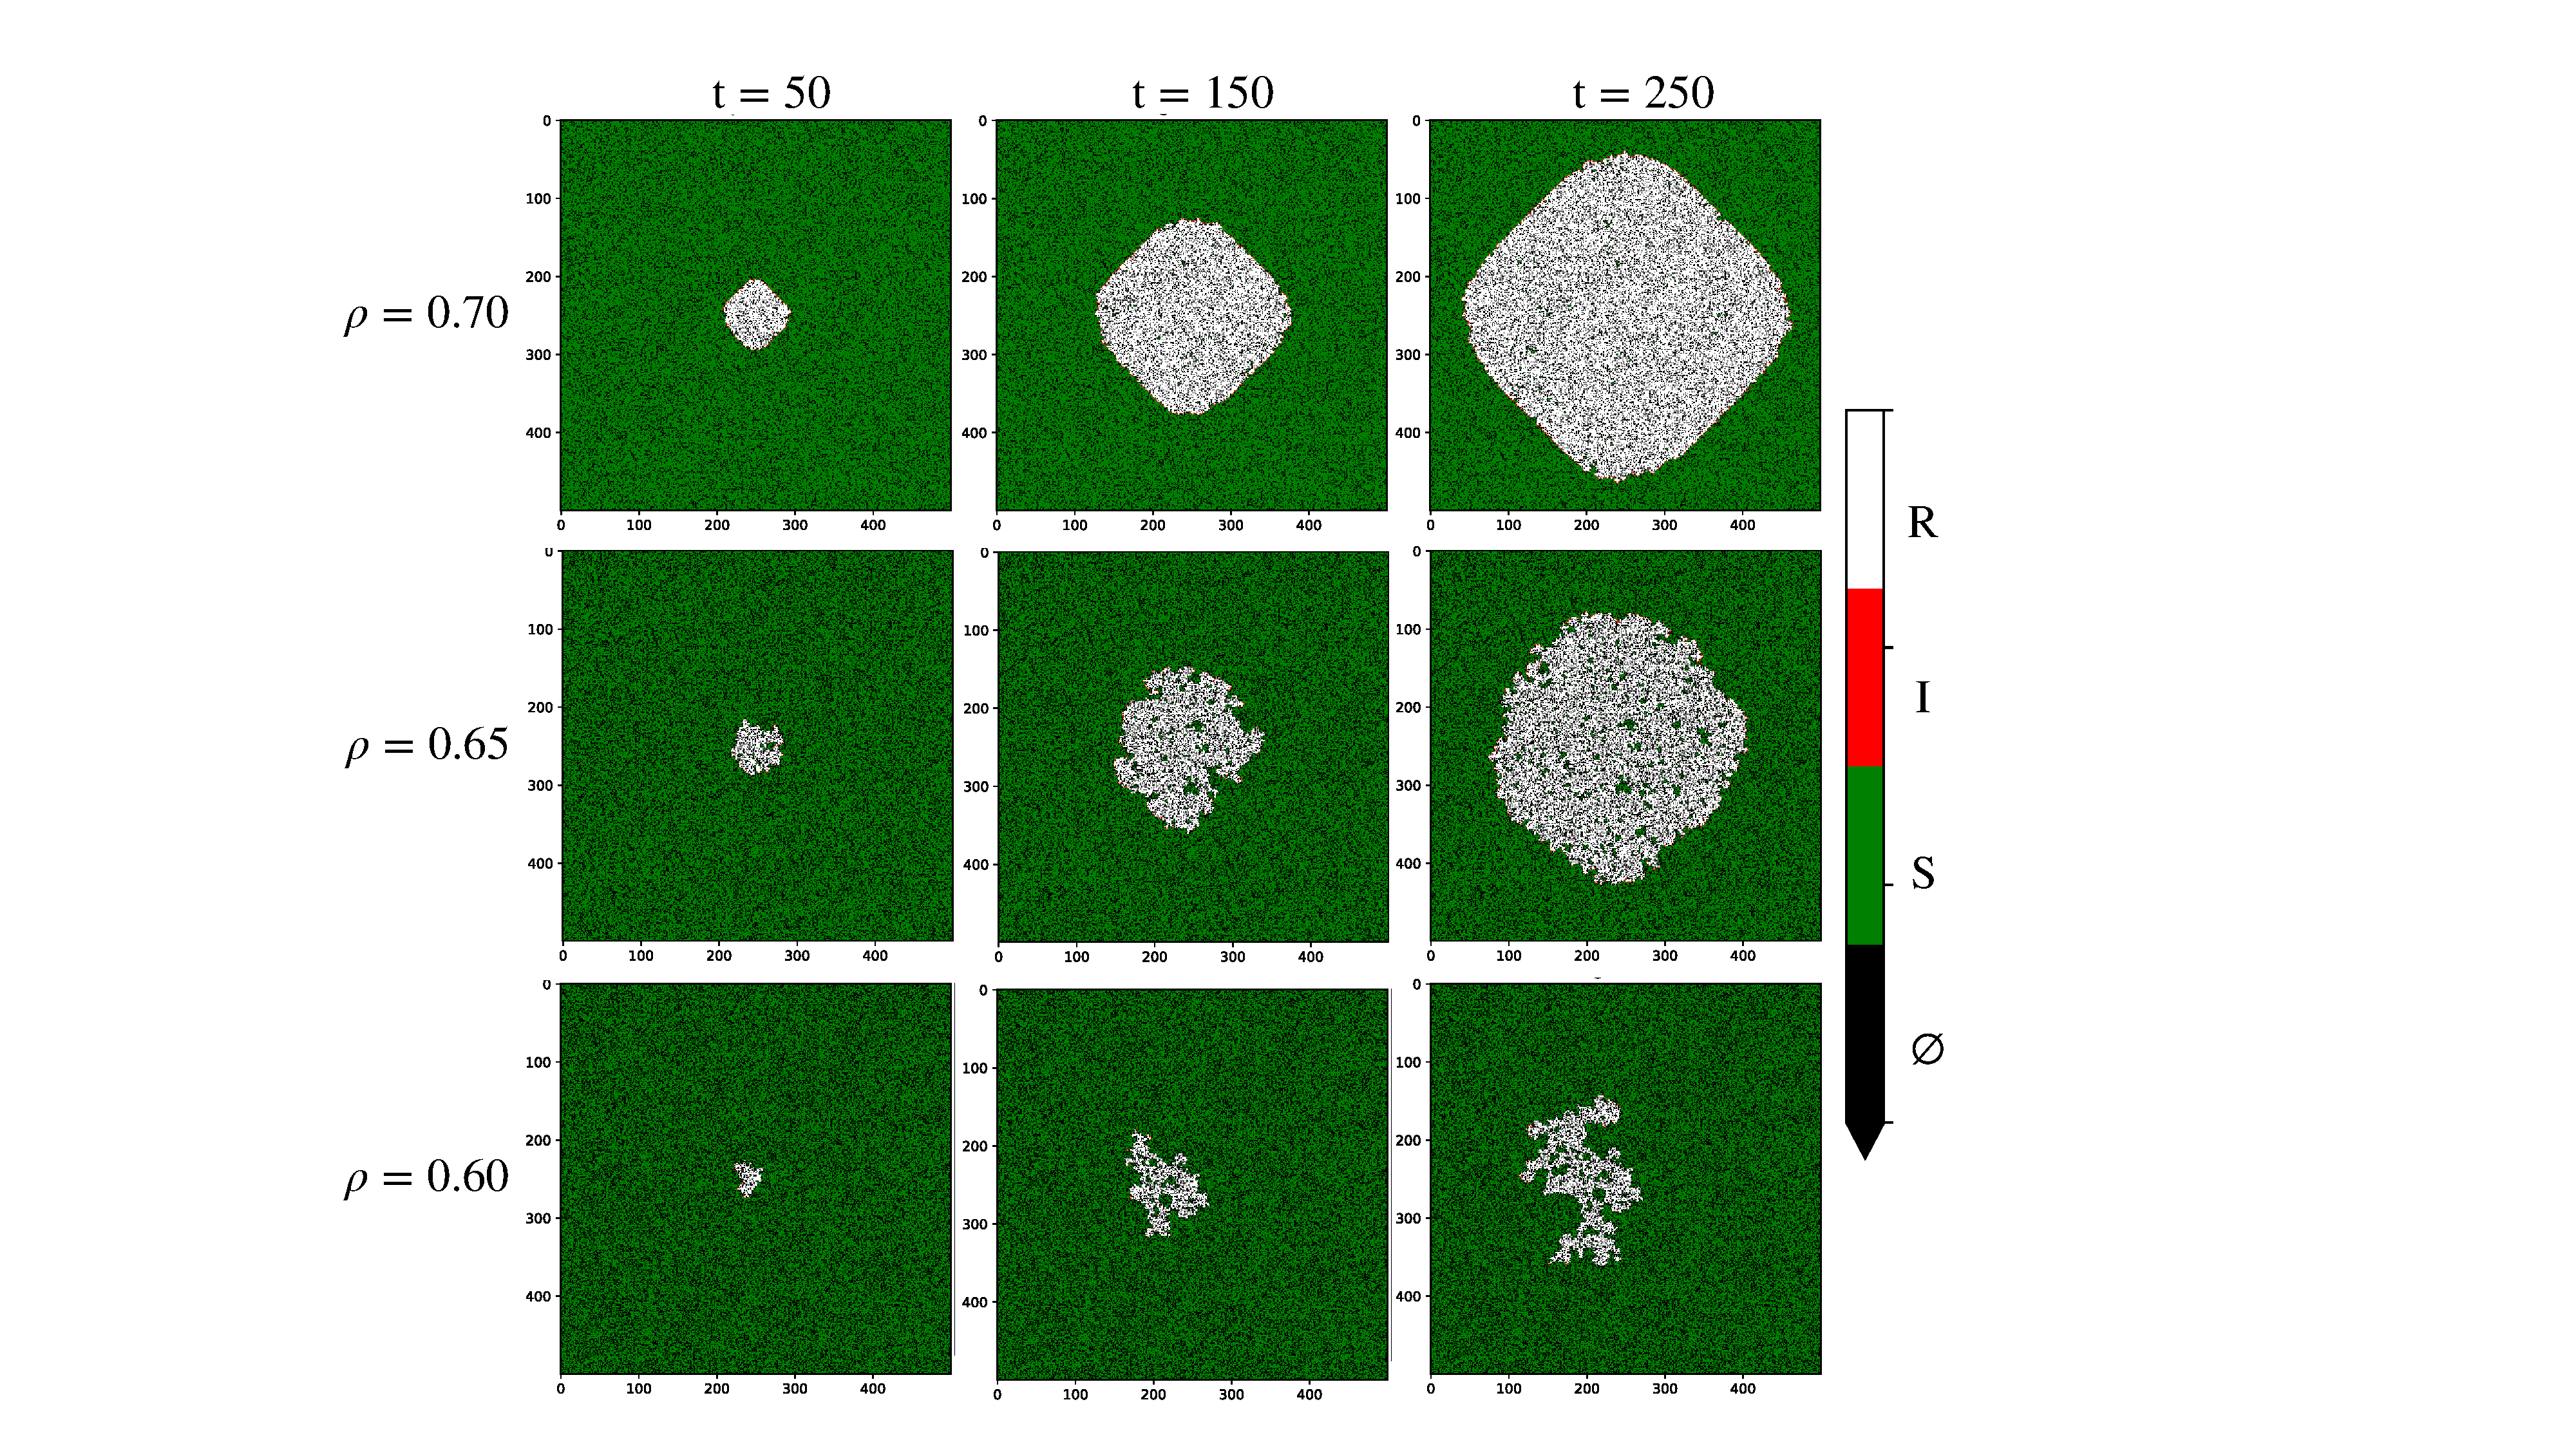
\includegraphics[scale=0.25]{chapter2/figures/figure1.pdf}
    \caption{The simulations of the $SIR$ model with parameter values of $\alpha = 0.10$ and $\beta = 0.35$.}
    \label{fig:sir}
\end{figure}

These equations gave insight into how and why the number of infected individuals varied over time, shown in Figure \ref{fig:sir}; the susceptible field (in green) begins to decrease as the  infected population (in red) rises, infected hosts are then removed (shown in black) until there are no hosts remaining to infect and the system reaches an equilibrium. Crucially this model displays a `threshold'. It was a long standing mystery as to why some outbreaks ensue for a time before coming to an halt whereas others continued for long-periods of time leading to wide-spread devastation i.e. an epidemic. Stability analysis of the $SIR$ model demonstrated the existence of a threshold $R_0$ given by:

\begin{equation}
    R_0=\frac{1}{N_0} \frac{\beta}{\alpha}
\end{equation}

where $N_0$ is the population size. The quantity $R_0$ is named the basic reproduction number and signifies the number of secondary infected cases which result from a single infected individual within a completely susceptible population. A threshold is defined by:
\[
  R_0=\begin{cases}
              Epidemic >1\\
              Extinction <1
            \end{cases}
\]

 It is clear to see the  model of $SIR$ is a vast simplification of the real process, however, it provides a starting place and can be generalised to include other categories such as `exposed'. Broadly speaking, epidemic thresholds are a crucial aspect of disease transmission and we will be discussed in detail throughout this thesis. There are various alternate mathematical and computational formulations of diseases \citep[see][]{review_} and we will proceed to review a selection of modelling paradigms associated with plant-based diseases. 